% chapter2.tex (Chapter 2 of the thesis)

\chapter{Assessment of Harmonic Based Techniques and Repertoire}\label{ch:chapter2}

% //TODO: Talk about Pythagoras - https://trello.com/c/uo0AALKP/1-talk-about-pythagoras
% Goals for this chapter:

% 1. Explain sound production of stringed instruments.
% 2. Explain the way in which the techniques differ from standard sound production.
% 3. Explain the qualities of the techniques.
% 4. Explain the notation.

Harmonic based techniques invariably make use of the harmonic series in one way or another. 
The harmonic series is a sequence of tones in which the frequency of each is an integer multiple of the fundamental frequency. 
The earliest forms of tuning systems were based around these, but modern instruments are tuned using equal temperament. 
The pitch of sound on stringed instruments is determined via tension, effecting the speed (and consequently pitch) the string vibrates at. 
Altering the tension is most commonly achieved via fingerings on the instrument's fingerboard, but bow pressure can also play a part in pitch production (see \hyperref[sec:subharmonics]{subharmonics}).

The objective categorisation of techniques is a Sisyphean task due to the variability of the techniques, but general guidelines can be made; Dick's \emph{The Other Flute} makes good use of quantifying qualitative data about the properties of multiphonics.\autocite[84]{dickOtherFlute1989}
However, his categorisation is based upon the physical properties of the flute, in which altering fingerings can drastically change the resultant sound.
As such, his method of partitioning and evaluating each quality will be used to paint a full picture of the technique in \autoref{ch:chapter4}, using the descriptive prose found in Adler's \emph{The Study of Orchestration}.\autocite[]{adlerStudyOrchestration2002}


To be able to pass any judgement on the techniques, we must first understand these techniques' capabilities, limitations, qualities, considerations, and values. 
Without references to other composers' works or professional musicians' opinions, any implication of authority on what constitutes as `idiomatic' writing is baseless. 
As such, references to other works, and feedback from sightreading sessions with professional musicians will be used to support claims. 
Where no such references are available, it will be marked as the author's personal opinion. 
Even without any available references to substantiate compositions as idiomatic, their creation contributes to the literature of the techniques, and thus can be used if not as an example, a warning on what not to do. 

All of the techniques covered in this exegesis involve the excitation of a string instrument's string in a non-standard way. 
A small amount of knowledge of the physics behind these techniques is required in order to understand the methods used to create these techniques.
Understanding the conditions under which these techniques are produced will help composers and performers alike realise the techniques' potential accurately and idiomatically.

Strings create sound via the Helmholtz motion, which is a cycle where the string sticks and slips along the bow.\autocite[]{wolfeBowsStrings}
Rosin is applied to bows in order to ensure the static friction of the bow is greater than the kinetic friction, allowing the string to stick to the bow better.

Benade describes it as such: 
\begin{quotation}
  `When the bow is placed on the string and drawn to one side, the string sticks to the bow, which pulls it aside until the elastic restoring force produced by the string tension becomes large enough to break the string loose from the bow.
  It now swings back in much the same way it would after slipping off the plectrum of a harpsichord jack; there is, however, a small amount of damping produced by the rapid (and therefore low-friction) sliding of the string against the steadily moving bow hair.
  At the end of its backward swing the string will come to rest and then recommence its motion in the direction of the bow velocity'\autocite[516]{benadeFundamentalsMusicalAcoustics1990}
\end{quotation}
% When the bow grabs the string, it carries it along, the kink traveling to the end point (i.e. the bridge) and then reflecting back, returning towards the bow.
% When it reaches the bow, the tension acts to pull it off the bow, breaking free and sliding back due to the low kinetic friction, propelled in the opposite direction by momentum.
Typically, the vibration of the string governs the cycle, and therefore the cycle of stick and slip on the bow has the same period as the vibration of the string.\autocite[]{wolfeBowsStrings}
Guettler et.\ al state that two conditions must be met in order to maintain Helmholtz motion;
\begin{quotation}
  (1) during the stick phase the bow force must be high enough to avoid premature slipping of the string, and 

  (2) the bow force must be low enough that the circulating Helmholtz corner can trigger the release of the string at the initiation of the slip phase.
\end{quotation}

When the bow drags the string too far, raucous motion is produced, which is recognisable as the sound produced by an amateur violinist.
Under the right conditions, \hyperref[sec:subharmonics]{subharmonics} are produced.

For the purposes of brevity, these harmonic-based extended techniques will simply be referred to as `techniques' throughout the paper, except for when differentiation between standard techniques is needed.
\emph{Normale} will be used throughout this exegesis to denote an arco bow stroke, with no modifying techniques.
% Harmonics will refer to the string technique, and partials will refer to the integer multiples of the fundamental.

% Provide an overlay of the techniques and explain how they work, the general benefits and such.
% \subsection{Research statement/problem}
% Techniques are under-developed and/or under-used.

% \subsection{Aim and scope of thesis}
% Examples of use in current literature will support use-case scenarios, dearths of usage will support the fact that they are underused.

% \subsection{Significance of work}
% The production of technique and its uses.
\newpage
\section{Subharmonics}\label{sec:subharmonicsDiscussion}
% TODO: Explain subharmonics - https://trello.com/c/HP0b1P3h/2-explain-subharmonics
First discovered by Mari Kimura, subharmonics are a type of overpressure which produces a sound lower than the fundamental.\autocite{kimuraHowProduceSubharmonics1999} 
They are also known as Anomalous Low Frequencies (ALFs), but Kimura argues that the predictable nature of them makes the name a misnomer.\autocite[]{kimuraHowProduceSubharmonics1999}
As such, they will only be referred to as subharmonics in this exegesis.
Subharmonics are produced when the bow is drawn across the string with an excessive amount of pressure.
The drag of the bow twists the string, creating torsional oscillation. 
Under the right conditions, these can interact with the string to produce an identifiable pitch lower than the fundamental.\autocite{Subharmonics2006}

The physics of how subharmonics are produced are not entirely understood as of time time of publication, although many inroads have been made.\footnote{Readers interested in learning more about the physics behind them should find the works of Guettler to be an excellent starting point.}\autocite[]{guettlerBowedStringDevelopment2002}
The exact details fall beyond the scope of this thesis, as composers and performers simply need to know the methods and characteristics of their production, rather than the science behind it.
Botting describes the technique as ``using bow placement, overpressure and a steady stroke to access various partials of the subharmonic series which exists in inverse to the harmonic series, ‘beneath’ the fundamental as it were''.\autocite[16]{bottingDevelopingPersonalVocabulary2019}
Subharmonics were initially thought to belong to the undertone series, a reflection of the harmonic series in which the fundamental frequency is \emph{divided} by integers, rather than multiplied.\autocite[]{shaahinmohajeriEqualdivisionsoflengthEdl240edo2019}
The pitches that can be produced do not follow any discernable ratio based pattern.\autocite[]{guettlerWaveAnalysisString1994}
As such, subharmonics strictly speaking are not a harmonic based technique, but remain within the scope of this thesis due to the misinformation surrounding them, and the prevailing similarities with harmonic techniques.

Subharmonics share a common relative with woodwind and brass instrument in pedal tones.
They operate in similar ways, though the method of production differs greatly, and the reliability of production of subharmonics is much lower than the equivalent on brass instruments.
Because of these commonalities, it is not unreasonable to make comparisons between subharmonics and its equivalents, especially in regards to notation and implementation in works.


Subharmonics represent an incredible opportunity for solo string repertoire. 
On higher pitched instruments, their use can provide harmonic support (particularly in cadenza passages) and extend the range of the instrument. 
On lower pitched instruments, subharmonics function better as a timbral mechanic, much like overpressure. 
One of the newest string techniques, subharmonics are still in their comparative infancy, and their notation has not been formalised. 

Subharmonics are explored in my works \nameref{sec:bassPiece}, and \nameref{sec:violaPiece}.


\subsection{Subharmonics in the literature}

One of the most significant contributions to the literature is Kimura's article `How To Produce Subharmonics', in which she details specific methods in which one can promote the production of subharmonics, making them easier.\autocite[]{kimuraHowProduceSubharmonics1999}
Notably, she found that older strings are more sympathetic to the production of subharmonics, theorised to be due to the buildup of fats on the string.
Adding twists to the string may also help (or hinder) the production of subharmonics, as shown in \autoref{tab:twistTable}.\autocite[]{kimuraHowProduceSubharmonics1999}

\begin{table}
  \centering
  \caption{Relation between twists in string and resultant subharmonics}\label{tab:twistTable}
  \begin{tabular}{llllllll} 
  \toprule
  \multicolumn{1}{r}{} & \multicolumn{1}{c}{1/2} & \multicolumn{1}{c}{1} & \multicolumn{1}{c}{2} & \multicolumn{1}{c}{3} & \multicolumn{1}{c}{4} & \multicolumn{1}{c}{5} & \multicolumn{1}{c}{6}  \\ 
  minor 2nd            & x                       & x                     &                       &                       &                       &                       &                        \\
  major 2nd            & x                       & x                     &                       &                       &                       &                       &                        \\
  minor 3rd            & x                       & x                     & x                     &                       &                       &                       &                        \\
  major 3rd            & x                       & x                     & x                     & x                     &                       &                       &                        \\
  perfect 4th          &                         &                       &                       & x                     & x                     &                       &                        \\
  diminished 5th       &                         &                       &                       &                       & x                     & x                     &                        \\
  perfect 5th          & x                       &                       &                       &                       &                       & x                     & x                      \\
  minor 6th            &                         &                       &                       &                       &                       &                       & x                      \\
  octave               & x                       & x                     & x                     & x                     & x                     &                       &                        \\
  \bottomrule
  \end{tabular}
  \end{table}

  Possibly the first person to make use of the technique, Crumb described what we know as subharmonics as `pedal tones'.\autocite{crumbBlackAngelsImages1971}
  Crumb makes use of square noteheads and a separate stave for the resultant pitch in \emph{Black Angels}, which makes the technique clear and readily understandable.\autocite[]{crumbBlackAngels1995}
  They are, however, purely timbral, and no recordings seem to treat them as subharmonics.
  
  \begin{figure}
    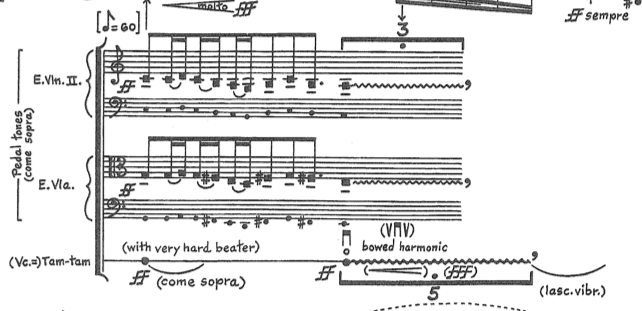
\includegraphics[width=\linewidth]{./resources/crumbBlackAngels.png}
    \caption{Excerpt from Crumb's \emph{Black Angels}, 4. `Devil Music'}\label{fig:Excerpt from Crumb's Black Angels}\end{figure}
  % TODO: Citation is needed for Crumb - https://trello.com/c/Rpypkzbm/4-citation-needed-for-crumb
  % TODO: Citation needed for pedal tones - https://trello.com/c/03arTJkS/5-citation-needed-for-pedal-tones

Sekulic describes subharmonics as:

\begin{quotation}
  [\ldots] a sound that sounds an octave lower than g string. 
  To produce this sound the use of bow is of great importance- the place, speed, and pressure. 
It is however extremely unsustainable and unpredictable, thus it is difficult to use it much in the compositions.\autocite[15]{sekulicYouHearMe2012}\end{quotation}

Sekulic erroneously claims that subharmonics are solely producible on the G string, and can only produce an octave. 
Kimura's work, and my own experiments on a contrabass show that subharmonics are possible on any string, and octaves, major sevenths, and minor seconds are all readily achievable without specialist practice.\autocite[]{kimuraHowProduceSubharmonics1999}



% \subsection{Notation of Subharmonics in the literature}



Gerard Grisey's \emph{Vortex Temporum} features overpressure, with a subharmonic of specifically a seventh.\autocite[]{griseyVortexTemporum}
He notates the subharmonic technique using a triangular filled notehead showing the intended pitch, along with a double down-bow, with an arrow above it, shown in \autoref{fig:Excerpt from Grisey's playing instructions for Vortex Temporum}. 
Somewhat abstracted out, this hides the intended effect behind symbols, and is slower to sight read.


\begin{figure}
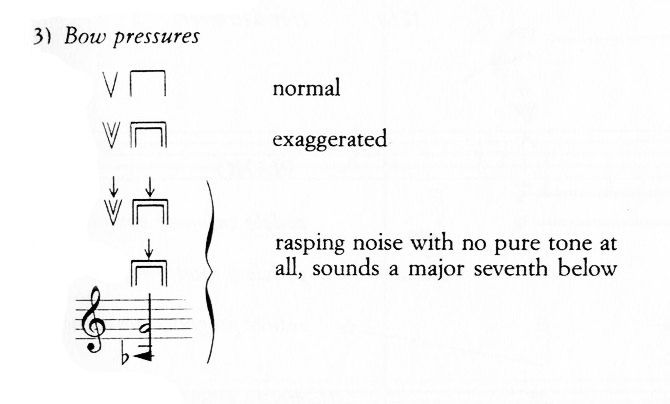
\includegraphics[width=\linewidth]{./resources/griseyVortexTemporum.jpg}
\caption{Excerpt from Grisey's playing instructions for \emph{Vortex Temporum}.}\label{fig:Excerpt from Grisey's playing instructions for Vortex Temporum}\end{figure}


Mari Kimura's \emph{Gemini} (\autoref{fig:Excerpt from Kimura's Gemini}) is an example of idiomatic usage of subharmonics on the violin.\autocite[]{kimuraGemini1992}
Kimura's notation practice of using a harmonic denoting the intended pitch below the fundamental is similar to the standard notation of harmonics, which Gould states is to ``write harmonics as the player will finger them''.\autocite[413]{gouldBars2011} 
Unfortunately, this method proved somewhat counterintuitive in practice, as the notation was too similar, and caused sight reading issues.\autocite[]{appleseedFeedbackExploratorySession2019}

  
\begin{figure}
  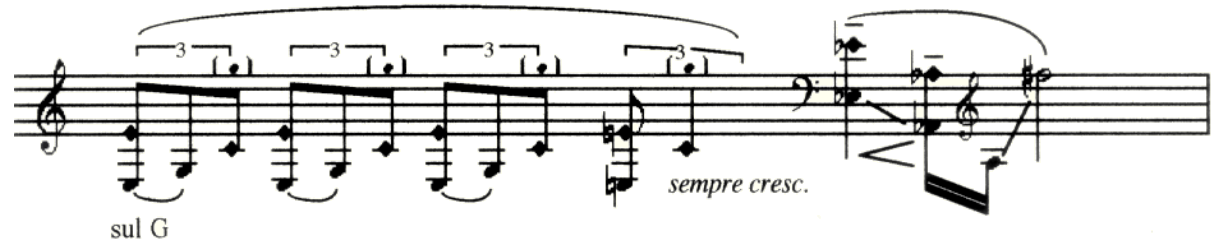
\includegraphics[width=\linewidth]{./resources/kimura_gemini.png}
  \caption{Excerpt from Kimura's \emph{Gemini}}\label{fig:Excerpt from Kimura's Gemini}
\end{figure}
% TODO: Citation needed for Gemini

The example used on Long's website, \emph{The Modern Double Bass} (\autoref{fig:LongNotation}) features a square notehead with the intended sound at pitch in a bracketed notehead, with harmonics and a technique line of `S.H'.\autocite[]{longSubharmonics2019}

\begin{figure}
  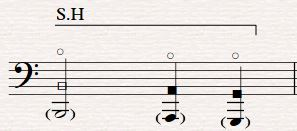
\includegraphics[width=\linewidth]{./resources/longSubharmonicNotation.jpg}
  \caption{Notation of subharmonics from Long's website, The Modern Double Bass}\label{fig:LongNotation}
\end{figure}

It is the author's opinion that this is somewhat redundant, as just square noteheads with the intended produced pitch would be enough to delineate the technique. 
The technique line is supernumerary, and it would only be advisable to use it in extended passages of uninterrupted subharmonics.

% TODO: reference risset and rowe - https://trello.com/c/wDhTSCzs/29-reference-risset-and-rowe

Rowe wrote a work for Kimura, and uses a regular notehead for fingering, with a square bracketed cue sized notehead, as seen in \autoref{fig:Excerpt from Rowe's Submarine}.\autocite[]{roweSubmarine1996}
% This combines the best of both worlds, keeping the score free from clutter when not needed.
\emph{Submarine} uses subharmonics early in the work as a contrast to the higher pitched material.
They are referred back to several times, either as a mechanism to further muddy the soundworld created by the digital processing, or to `clear the palette', the electronic audio cutting out leaving just the authoritative tone of the subharmonic.
Rowe makes use of the audio processing, recording the subharmonics and playing them back later; an economical way to use the technique, which can be unreliable.
Near the end of the work, Rowe immediately plays back the just-recorded subharmonic, overcoming the limitation of the subharmonic's inability to handle sustained durations through technology. 
It should be noted that Rowe uses notation that has fallen out of style to notate \emph{normale} harmonics, notating the fingering position with the diamond notehead, and the resultant pitch with a harmonic circle above it. 
Harmonic circles always denote resultant pitch, and are usually reserved for octave harmonics; the inclusion of the fingering obfuscates the intent.\autocite[420]{gouldBars2011}


\begin{figure}
  \includegraphics[width=\linewidth]{./resources/roweALFExcerpt.pdf}
  \caption{Excerpt from Rowe's \emph{Submarine}}\label{fig:Excerpt from Rowe's Submarine}\end{figure}

Jean-Claude Risset's \emph{Variants}, also written for Kimura, is a work that makes use of both subharmonics and digital processing of live sound.\autocite[]{rissetVariants1995}
It uses a separate stave for the subharmonics and digital processing, as seen in \autoref{fig:Excerpt from Risset's Variants}. 

\begin{figure}
  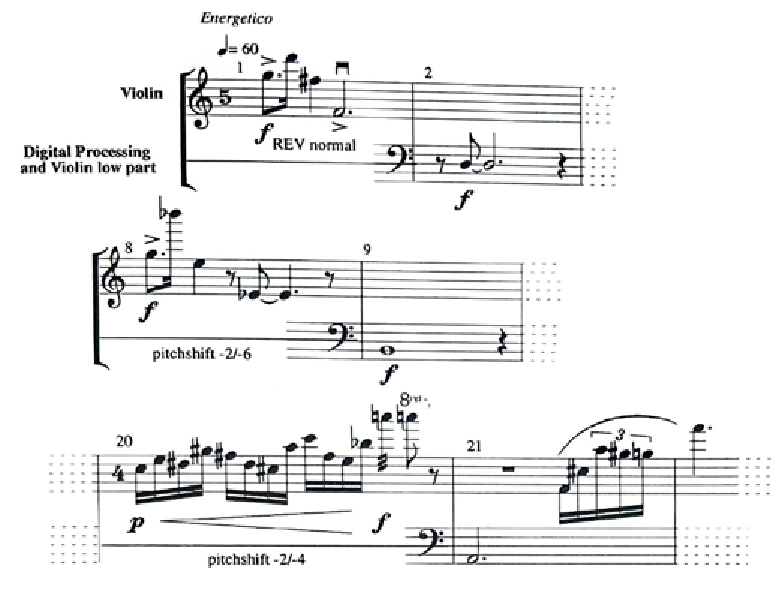
\includegraphics[]{./resources/rissetALFExcerpt.pdf}
  \caption{Excerpt from Risset's \emph{Variants}}\label{fig:Excerpt from Risset's Variants}\end{figure}

In \emph{Variants}, Risset uses digital processing software to create chords out of singular melodic lines on the violin.
This gives the impression of a full string section when the violin is playing fast \emph{normale} passages, and emphasises the raucous, harsh timbre when playing subharmonics.
They are used as a timbral device, rather than anything pitch based, with the longest subharmonic going for little more than two seconds, with three subharmonics appearing in the piece in total.


Botting uses a fingering stave, and two staves for the resultant pitch which also contains the technique information, denoted by `SH' and a diamond notehead (confusingly, the stave is called the `written pitch').\autocite[109]{bottingDevelopingPersonalVocabulary2019}
Apart from the technique text belonging attached to the stave that is performed, this is an acceptable method of showing resultant pitches when subharmonics are used in conjunction with harmonics.
Botting's score was included in the appendices of his thesis, but it is unclear if frontmatter was omitted; given that Botting performs the piece personally, it is not unreasonable to assume that the work was written solely for his own practice (and therefore required no explanation of the techniques).
This is, however, not acceptable for composers looking to use the technique in pieces performed by other people, and Gould is quite explicit in stating that all extended techniques must be covered in the frontmatter.\autocite[494]{gouldBars2011}

\begin{figure}
  \centering
  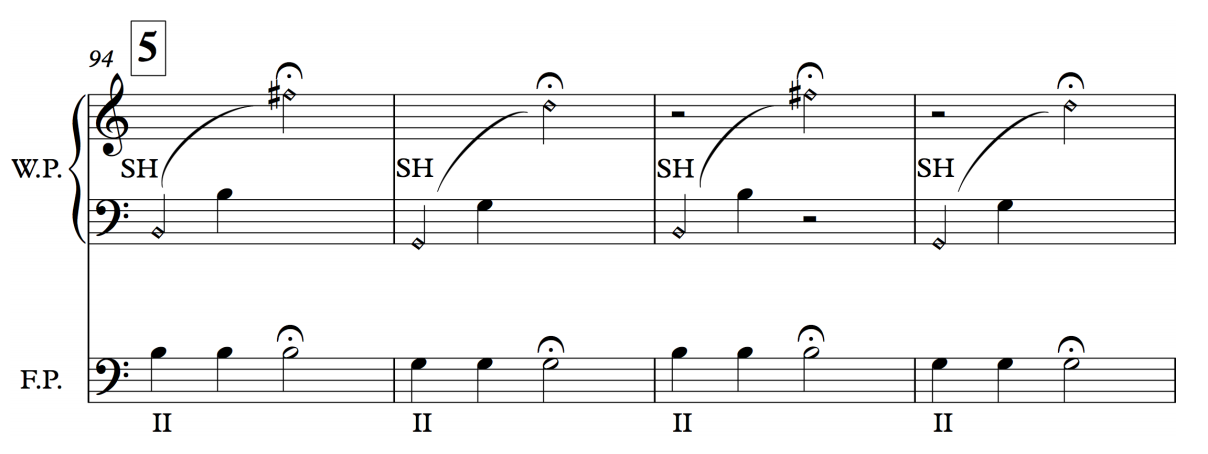
\includegraphics[width=\linewidth]{./resources/bottingStave.png}
  \caption{Excerpt from Botting's \emph{Heights and Depths} mm. 94--97}\label{fig:BottingMultiphonics}\end{figure}

This section of movement between subharmonics, \emph{normale}, and harmonics lasts for no more than seventeen bars, but is enough to recognise the compositional potential.
The textural movement from rough, gravely subharmonics through to pure harmonics, combined with the ascending pitch material gives a natural wedge shape to the phrase.
The effect is more pronounced on the harmonics that result in a major third interval and minor seventh at bars 102 and 103 respectively.
It then shifts into multiphonics, showing that these techniques can work in quick succession.\autocite[154--155]{bottingDevelopingPersonalVocabulary2019}

Through an examination of the literature, there appears to be a range of different notation methods and levels of understanding of the mechanics of subharmonics.

% Musicians are better at sight reading above the stave than below the stave, so unlike natural harmonics, the need to split into another stave to show the resultant pitch is likely to be more common for composers wishing to use subharmonics. 
% TODO: undefined - https://trello.com/c/SU5ZEEmJ/6-- Do I need a citation for "musicians are better at sight reading above the stave than below"?

\newpage
\section{Multiphonics}\label{sec:multiphonicsDiscussion}
% TODO: Explain multiphonics - https://trello.com/c/6vkcY6CO/7-explain-multiphonics

Multiphonics, also known as split tones, are `the simultaneous sounding of two or more harmonics on a single string'.\autocites[108]{fallowfieldCelloMapHandbook2009}[http://www.cellomap.com/index/the-string/the-left-hand.html]{fallowfieldCelloMap}
For the purposes of this exegesis, they will only be referred to as multiphonics.
An acoustical explanation for the production of multiphonics is still lacking, although it can be surmised that much like how octave harmonics can withstand a large margin of pitching error in order to activate, several partials' `tolerance zones' for activation overlap.\autocites[146]{fallowfieldCelloMapHandbook2009}{bloggsFeedbackContrabassSession2019}
Multiphonics are most commonly the domain of wind, and occasionally brass instruments, but they are an emerging technique in string writing, Turetzky writing about them in 1974.\autocite[138]{turetzkyContemporaryContrabass1974}
% They are produced when fingerings split the string between two natural harmonics, allowing for the string to resonate at multiple frequencies.
% TODO: Citation needed for explanation of physics of multiphonics - https://trello.com/c/EboMHDaN/8-citation-needed-for-explanation-of-physics-of-multiphonics
Multiphonics on stringed instruments are difficult, but with appropriate preparation and notation, are feasible. 
Production of multiphonics, as with wind instruments, is not guaranteed, and can be dependant on a variety of external factors, including the humidity, make of the instrument, bow used, and other variables that are outside of the control of a composer. 
% TODO: Citation needed for the factors leading to multiphonics - https://trello.com/c/9iC7EAXb/24-citation-needed-for-the-factors-leading-to-multiphonics
 


Multiphonics are explored in my piece for violoncello, \nameref{sec:celloPiece}, and contrabass work \nameref{sec:bassPiece}.

\subsection{Multiphonics in the literature}

Fallowfield explores multiphonic production on the cello in her thesis CelloMap comprehensively, with video recordings of all possible multiphonics and permutations, including pizzicati.\autocite{fallowfieldCelloMapHandbook2009} 
These are isolated, though, and give little indication to the difficulty of the multiphonics.

In Strange and Strange's \emph{The Contemporary Violin}, Tracy Silverman compares the sound to electronic feedback.\autocite[132]{strangeContemporaryViolinExtended2001}
Welbanks compares and contrasts between Fallowfield and Silverman's assessment of the technique, and concludes that Silverman believes that multiphonics are a predominantly left-hand technique, while Fallowfield argues for a more holistic view, with the bow.\autocite[161--164]{welbanksFoundationsModernCello}

Ashley John Long's `The Modern Double Bass' website serves a similar purpose as Fallowfield's CelloMap for the double bass.\autocite{longModernDoubleBass} 
He divides them into different categories as detailed in \autoref{tab:longTable}, some of which have more information and detail than others. 

\begin{table}[]
  \centering
  \resizebox{\textwidth}{!}{%
  \begin{tabular}{@{}ll@{}}
  \toprule
  \textbf{Type}                                      & \textbf{Description}                                                       \\ \midrule
  `Natural' multiphonics                             & Chart of different fingerings, similar to Fallowfield.                     \\ \midrule
  Pizzicato multiphonics                             & Description of technique, production, and result.                          \\ \midrule
  Textural multiphonics                              & Description of technique, production, result, and considerations.          \\ \midrule
  Multiphonics behind the bridge                     & Description of technique.                                                  \\ \midrule
  Artificial multiphonics                            & Chart of different fingerings, similar to Fallowfield.                     \\ \midrule
  Percussive multiphonics                            & Description of technique, production, result, and considerations.          \\ \midrule
  Timbral multiphonics                               & Description of technique.                                                  \\ \midrule
  Transformative multiphonics                        & Description and production of technique                                    \\ \midrule
  Multiphonics through Variations in Finger Pressure & Description of technique, production, result, considerations, and example. \\ \bottomrule
  \end{tabular}%
  }
  \caption{The different types of multiphonics according to Long}\label{tab:longTable}\end{table}

  Despite the varying degrees of detail, his work on cataloguing multiphonics is more in depth than many other resources.

 

\subsection{Notation of Multiphonics in the literature}

It should be noted that multiphonics are markedly different to the multiphonics of wind instruments due to the fingering systems.
While wind instruments achieve multiple tones by exploiting the construction of their instrument, string multiphonics are produced agnostic of specific fingerings.
As such, the challenges that string multiphonic notation face are different to wind instruments.
With no fingering chart necessary, string instrument multiphonics also have no frame of reference for what sounds can be expected to be produced.
String instruments also are not solely monophonic instruments, so notating the resultant multiphonic on the stave produces confusing results.
Compounding this issue, string instrument multiphonics are a subset of harmonics, which use a different notehead to denote the fingering pressure difference.
This means that any resultant pitches would need to be notated with regular noteheads, to discern the fingering pitch from the resultant.
Therefore, another system of denoting multiphonics must be used, as the existing wind literature is not suited for the purpose.

Strange and Strange discuss multiphonics at length, but lacked the literature necessary to form an opinion regarding their notation, stating that ``to our knowledge these string multiphonics have never been notated''.\autocite[132--134]{strangeContemporaryViolinExtended2001}
They present a potential notation system as seen in \autoref{fig:strangeMultiphonicNotation}, and justify it thus;

\begin{quote}
  The effect is a variant of an open harmonic, so it is logical to begin with that symbol- a small circle over the sounding pitch. 
  The timbral characteristics of the multiphonic is a distortion, or breaking up of the various other partials, much like a true \emph{sul ponticello}.\autocite[134]{strangeContemporaryViolinExtended2001}
\end{quote}

  \begin{figure}
    \centering
    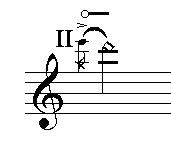
\includegraphics{./resources/strangeMultiphonicNotation.pdf}
    \caption{Strange and Strange's suggested multiphonic notation.}\label{fig:strangeMultiphonicNotation}\end{figure}

Buene uses a chart of diamond noteheads with their corresponding intended multiphonic in the score for his work for two double basses, \emph{Blacklight}.\autocite[39--42]{thelinMultiphonicsDoubleBass2011}
It mimics Fallowfield's charts of corresponding nearby quartertones, though the diamond notehead is already used in common repertoire for harmonics, not an extended technique. 
This has the potential to cause confusion, and could be easily avoided with a symbol or `M' denoting the special quality of the multiphonic, and Gould warns against such repurposing of existing symbols.\autocite[494]{gouldBars2011}

\begin{figure}
  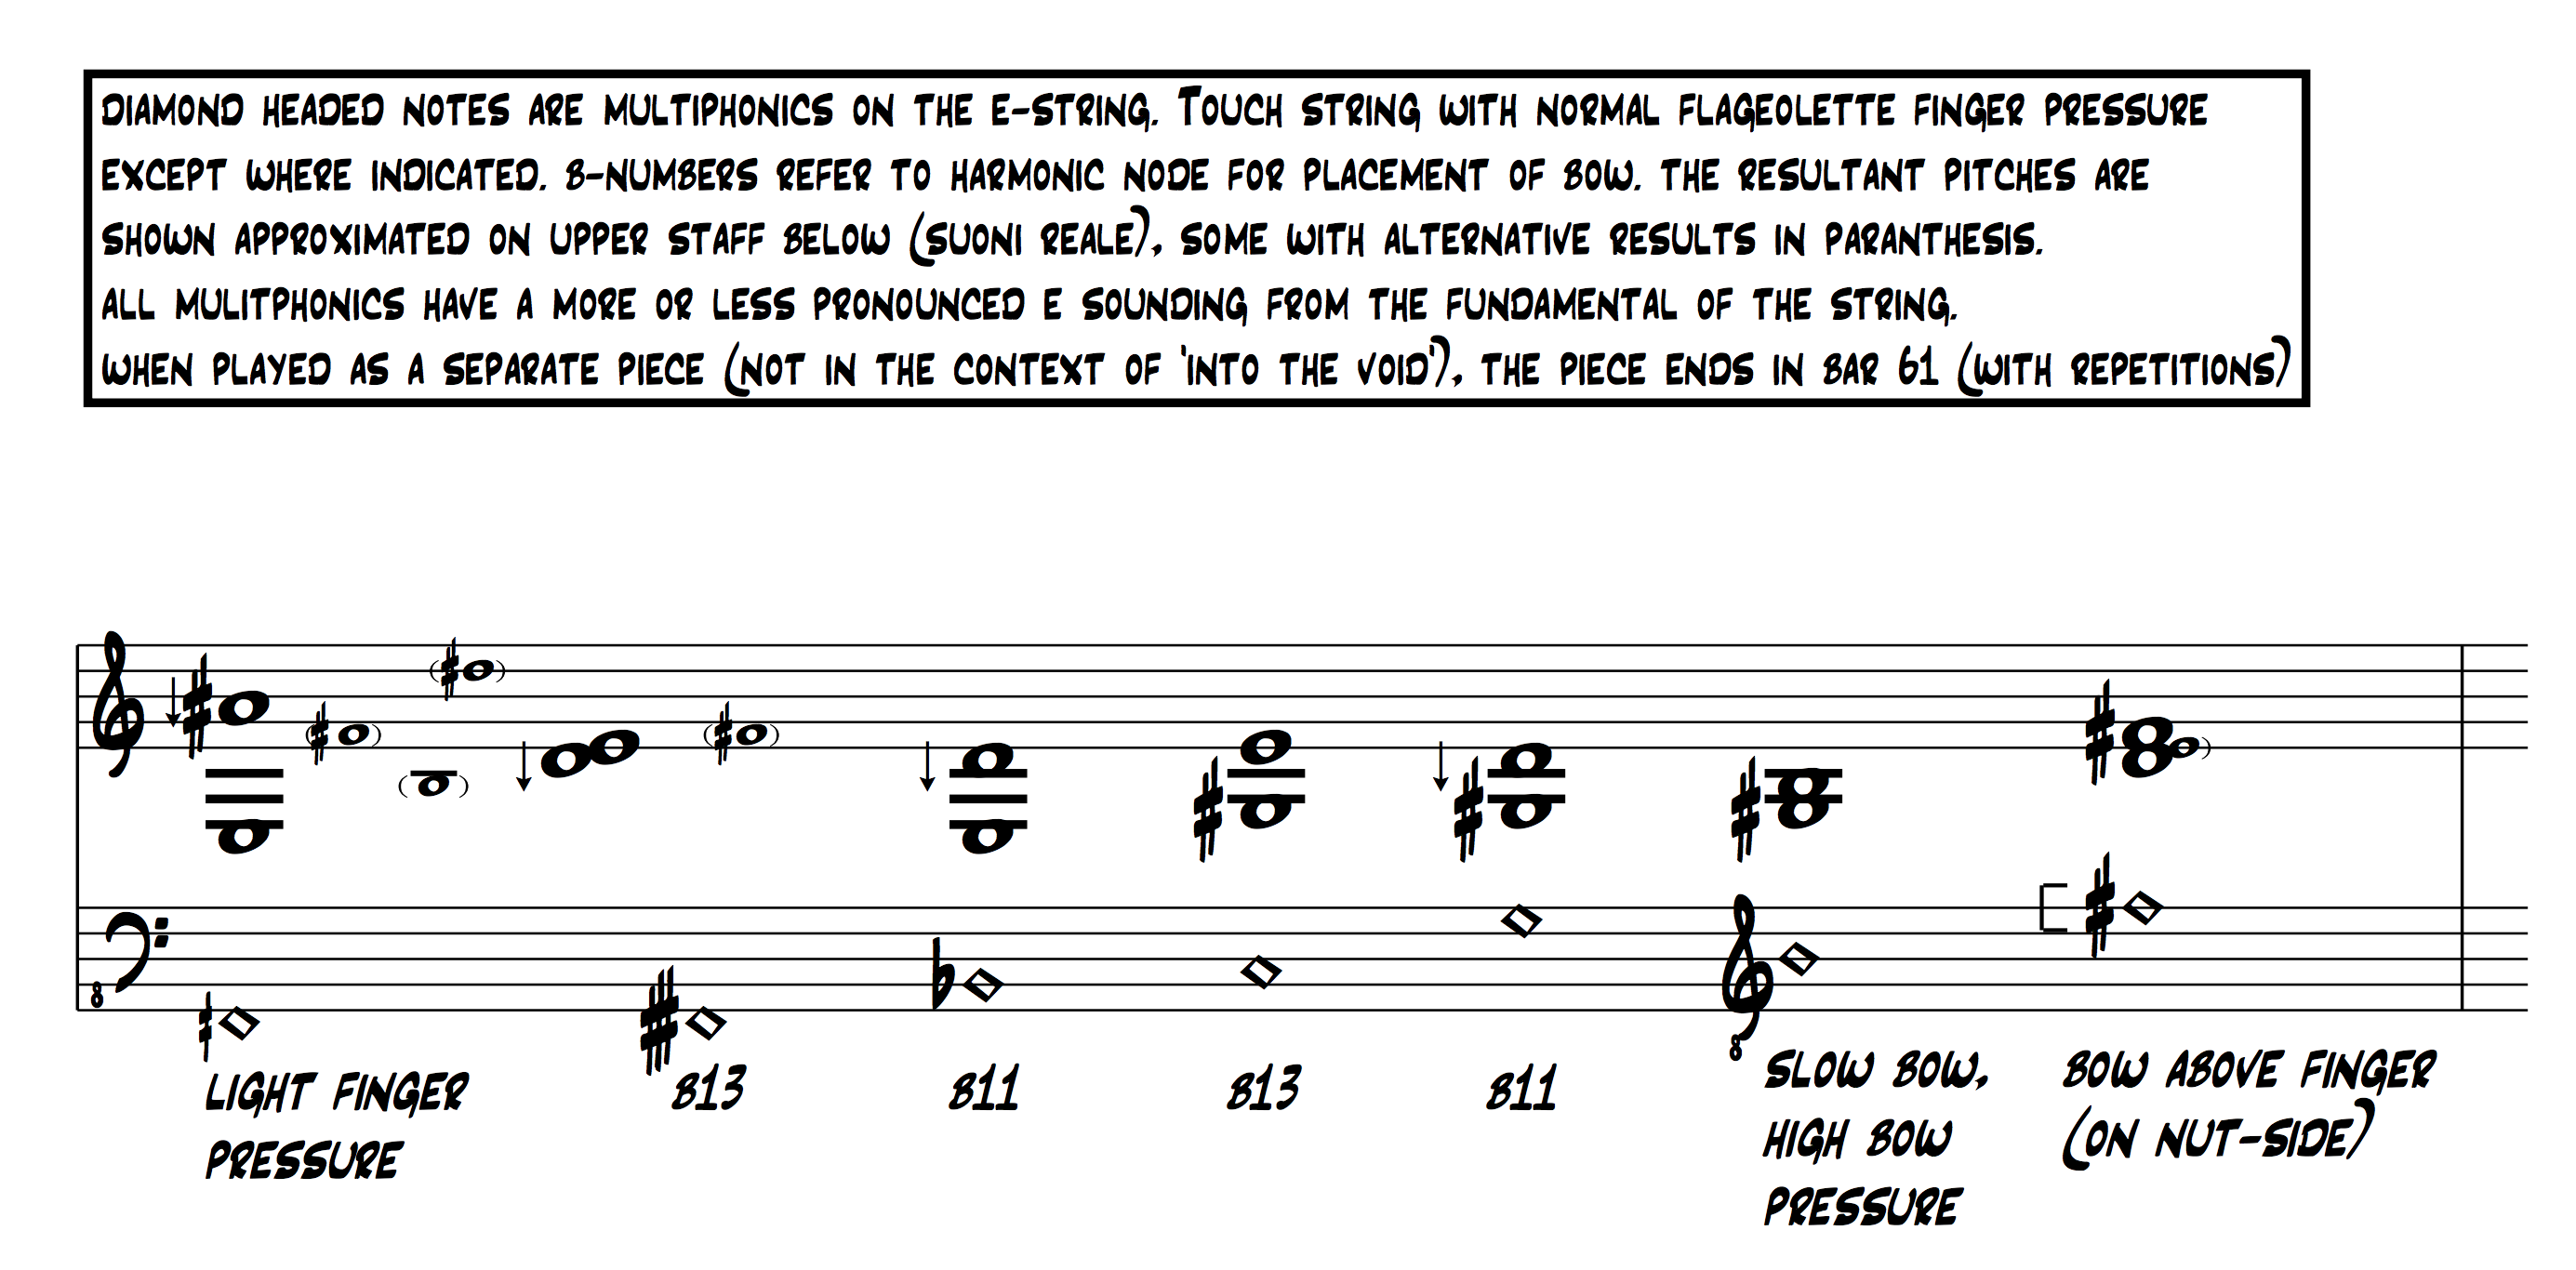
\includegraphics[width=\linewidth]{./resources/bueneMultiphonicNotation.png}
  \caption{Excerpt from Buene's \emph{Blacklight}.}\label{fig:Excerpt from Buene's Blacklight}\end{figure}

Thelin's thesis on double bass multiphonics states:
\begin{quotation}
    Multiphonics are always notated with the harmonic diamond sign, in tablature notation
    indicating finger positions rather than musical pitches. I suggest using the symbol M. above or
    below the note to indicate that it is a multiphonic sound, together with the indication on which
    string to play the note (in Roman numerals).\autocite[6]{thelinMultiphonicsDoubleBass2011}
\end{quotation}


\begin{figure}
    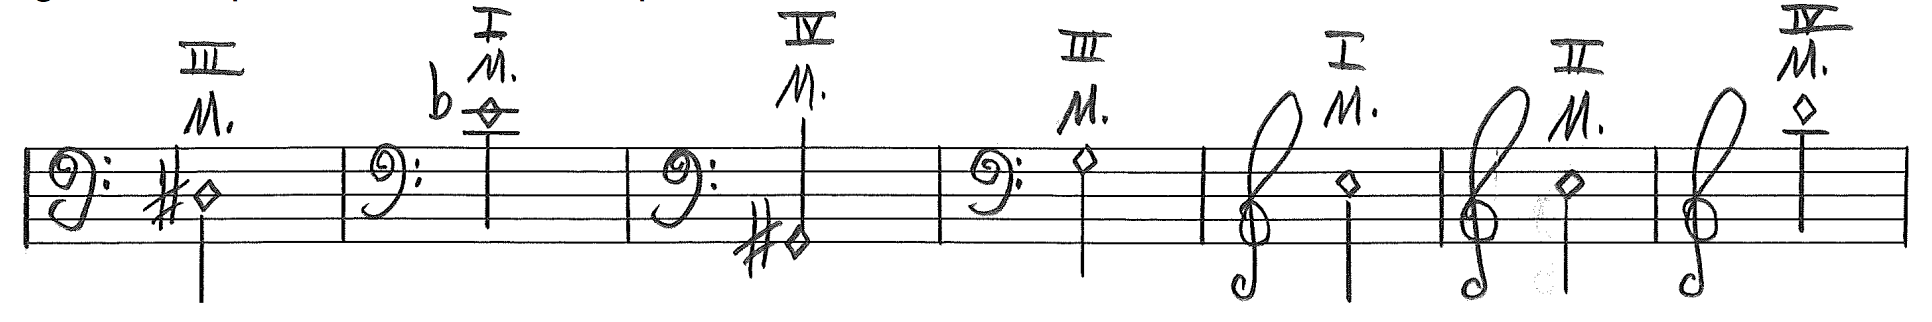
\includegraphics[width=\linewidth]{./resources/thelinMultiphonicNotation.png}
    % TODO: What is an excerpt from a thesis called? - https://trello.com/c/6xHaco1o/10-what-is-an-excerpt-from-a-thesis-called
    \caption{Excerpt from Thelin's thesis.}\label{fig:Excerpt from Thelin's thesis}\end{figure}
%   TODO: Reword Fallowfield dual harmonic positions
His notation, seen in \autoref{fig:Excerpt from Thelin's thesis}, is a somewhat less sophisticated version of Fallowfield's, lacking the tuning information necessary to produce the multiphonic. 
It should also be noted that Gould warns against technique text being placed below the stave.\autocite[492]{gouldBars2011}

Fallowfield proposes the form of notation seen in \autoref{fig:fallowfieldExampleMultiphonicNotation}, stating:
\begin{quotation}
  [\ldots] it is necessary to indicate both the left-hand finger position and the pitch content. 
  The left-hand finger touches the string above the node of the highest harmonic that contributes to the multiphonic, so the finger position is always that of the highest harmonic in the group. 
  I suggest notating finger position with the rhombus that is usually used for harmonic finger pressure. 
  The pitch of the contributing harmonics could be notated in brackets or on a separate stave. 
  It is necessary to indicate which string the multiphonic should be played on and helpful to use the indication ‘M’ for multiphonic.\autocite[http://www.cellomap.com/index/the-string/multiphonics-and-other-multiple-sounds.html]{fallowfieldCelloMap}
\end{quotation}

\begin{figure}
  \centering
      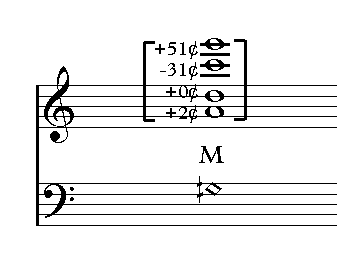
\includegraphics{./resources/fallowfieldExampleMultiphonicNotation.pdf}
      % TODO: What is an excerpt from a website called? - https://trello.com/c/04ESsMtJ/9-what-is-an-excerpt-from-a-website-called
      \caption{Fallowfield's proposed notation.}\label{fig:fallowfieldExampleMultiphonicNotation}\end{figure}

This notation is effective, although omits the indication of which string the multiphonic should be played on as she specified.

% Due to the symmetry of the production of harmonics on the string, Fallowfield specifies both upper and lower positions necessary to produce the same multiphonic.\autocite[index/the-string/multiphonics-and-other-multiple-sounds/fingeringcharts.html]{fallowfieldCelloMap}
% \begin{figure}
%     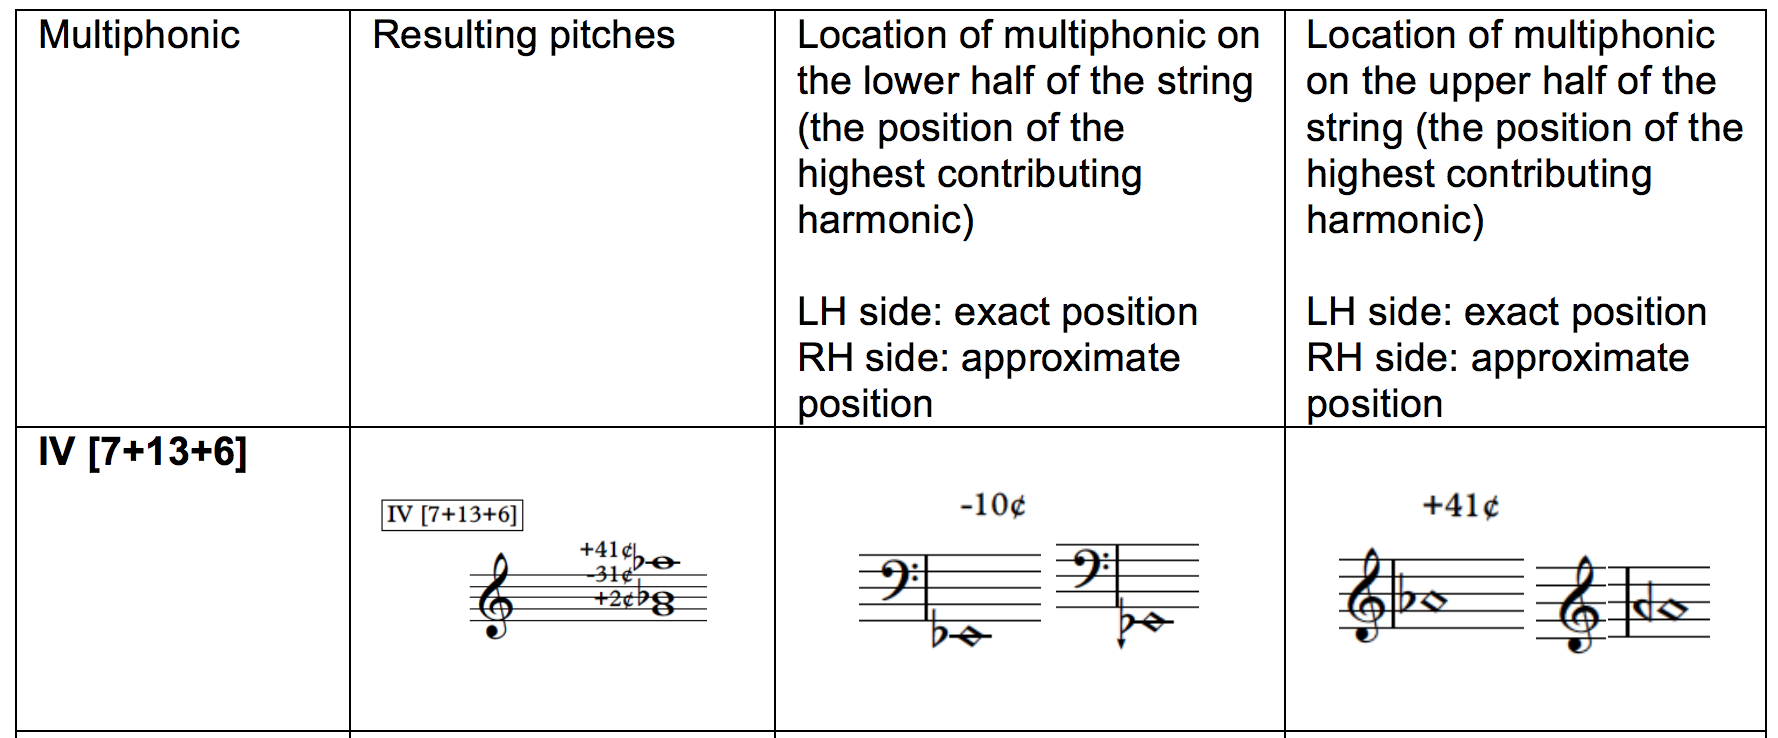
\includegraphics[width=\linewidth]{./resources/fallowfieldMultiphonicFingering.png}
%     % TODO: What is an excerpt from a website called? - https://trello.com/c/04ESsMtJ/9-what-is-an-excerpt-from-a-website-called
%     \caption{Excerpt from Fallowfields's website.}\autocite[]{fallowfieldCelloMap}
% \label{fig:Excerpt from Fallowfields's website}
%   \end{figure}

We can see this in practice in Oliver Thurley's work for solo contrabass, \emph{yet another example of the porousness of certain borders}, where he adds another stave showing the intended pitches to be produced.\autocite{thurleyAnotherExamplePorousness2014}

  \begin{figure}
    \centering
    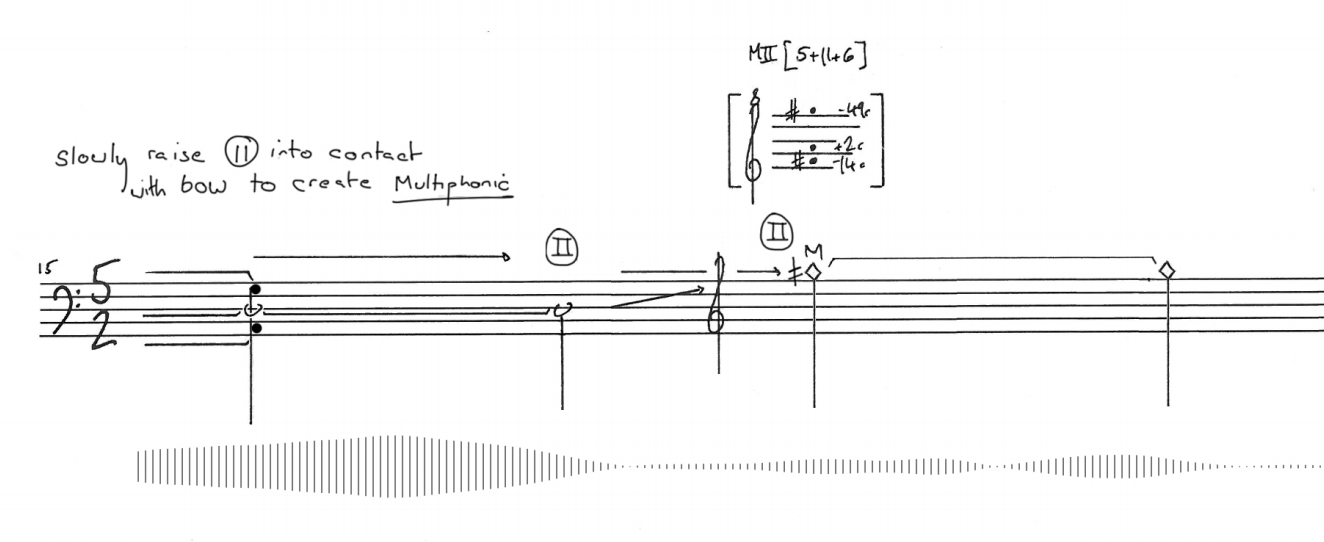
\includegraphics[width=\linewidth]{./resources/thurleyMultiphonicNotation.png}
    % TODO: What is an excerpt from a piece called? - https://trello.com/c/E9QqxFt0/12-what-is-an-excerpt-from-a-piece-called
    % TODO: Quotation marks in figure labels? - https://trello.com/c/HLJwnAwa/11-quotation-marks-in-figure-labels
    \caption{Excerpt from Thurley's \emph{yet another example of the porousness of certain borders}}\label{fig:Excerpt from Thurley's `yet another example of the porousness of certain borders'}\end{figure}

Thurley embraces the fragility of these multiphonics, and uses their variability as a feature, rather than a hindrance. 
Slow, quiet transitions between multiphonics, double-stopped harmonics, and other extended techniques make the occasional unintentional destabilisation of a multiphonic a point of textural interest, rather than a flaw.

Botting uses a diamond notehead for fingering, and a stave above containing the resultant pitches as diamond noteheads with an `M' above them, as shown in \autoref{fig:bottingMultiphonics}.\autocite[35]{bottingDevelopingPersonalVocabulary2019}

\begin{figure}
  \centering
  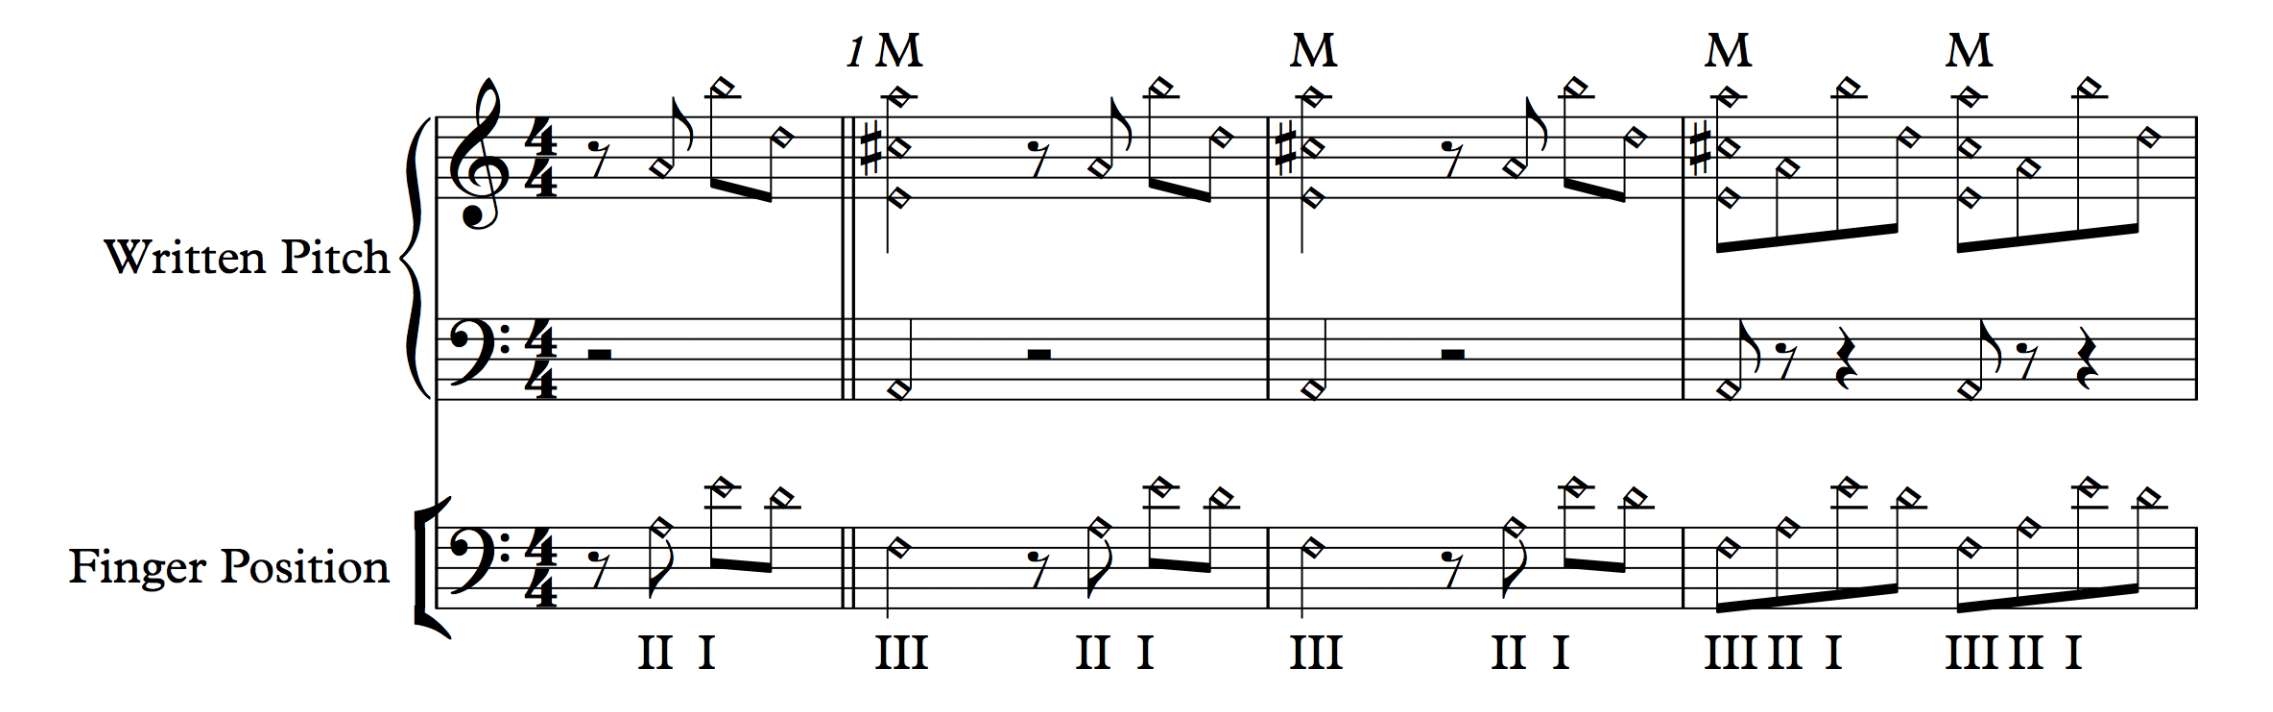
\includegraphics[width=\linewidth]{./resources/bottingEtudeExample.png}
  \caption{Excerpt from Botting's \emph{Study in Harmonics and Multiphonics no. 1}}\label{fig:bottingMultiphonics}\end{figure}

The \emph{Study in Harmonics and Multiphonics no. 1} repeats the melodic material, and we see that the multiphonic not only slots in as something that can be played at an \emph{andante rubato}, but we see the bow move across the strings, shifting from D to G to a multiphonic on the A string.
It should be noted that Botting produced this notation system without reference to the preexisting works of Fallowfield.
This suggests that the use of an `M' to specify a multiphonic is a relatively intuitive way of conveying the information (preceded, of course, by front matter explaining the technique).

It becomes apparent through the examination of the literature surrounding multiphonics that they are still an emerging technique, but are not shrouded in mystery or disinformation as subharmonics are.

\newpage
\section{Half-Harmonics}\label{sec:halfHarmonicsDiscussion}
% TODO: Explain half-harmonics - https://trello.com/c/0v3lKvmZ/25-explain-half-harmonics
Half-harmonics is a term assigned to the fingering pressure found somewhere in between a regular note and harmonic. 
The technique is not difficult to produce, and the resultant sound is not dissimilar to the fragility of a multiphonic, producing both the fundamental pitch, and the harmonic. 
It should be noted that the half-harmonic is a modifying left-hand technique; it can be applied to multiphonics (although the resultant sound would likely be more noise than discernably either of the two techniques), but is not compatible with subharmonics due to the bow pressure needed to produce subharmonics eliminating the possibility of half-harmonics being produced.
The terminology has not been formalised, but is most widely known as half-harmonics, although some works describe the technique without ascribing a name.

Half-harmonics are explored in my work for violin, \nameref{sec:violinPiece}.

\subsection{Half-harmonics in the literature}
Half-harmonics, like the other techniques covered in this exegesis, have relatives in the wind and brass literature. 
Half-fingered and half-valved techniques appear in the respective nomenclature, and share common attributes of speaking poorly with bleedover into partials with the half-harmonic technique.
Unlike multiphonics, the mechanical production of the technique is not dissimilar to the wind and brass facsimiles; all three families' respective techniques revolve around pressing almost to the point of a \emph{normale} sound, but not quite, resulting in a pinched sound.
Because of this, it is not unreasonable to draw parallels between the half-valved and fingered literature, and half-harmonic literature. 

Half-harmonics do not feature heavily in the literature, with the most notable work being Sciarrino's 6 Caprices for solo violin.\autocite{sciarrinoCapricciViolino1976} 
It should be noted that Sciarrino wrote these in response to Paganini's caprices. 
They appear to take the same approach to composing in the same philosophy as New Complexicists, in the sense that the written score is the Platonic ideal, and that approximations are all that are expected.
This is supported by the fact that many performers play them as harmonics.\autocite[]{appleseedFeedbackExploratorySession2019}

% TODO: add references for sciarrino claims - https://trello.com/c/7DtUyFWz/31-add-references-for-sciarrino-claims

Lachenmann also makes use of them, and states it is
\begin{quotation}
  [\dots] `important not to produce any harmonics here; the result should be a veiled, almost immaterial and hardly perceptible coloring of the dominating string sound produced by the stopped note'\autocite[foreword]{lachenmannMusikFurStreichquartett1972}
\end{quotation}
% Half-harmonics are used typically as a colourant, rather than a feature technique, and 

\begin{figure}
  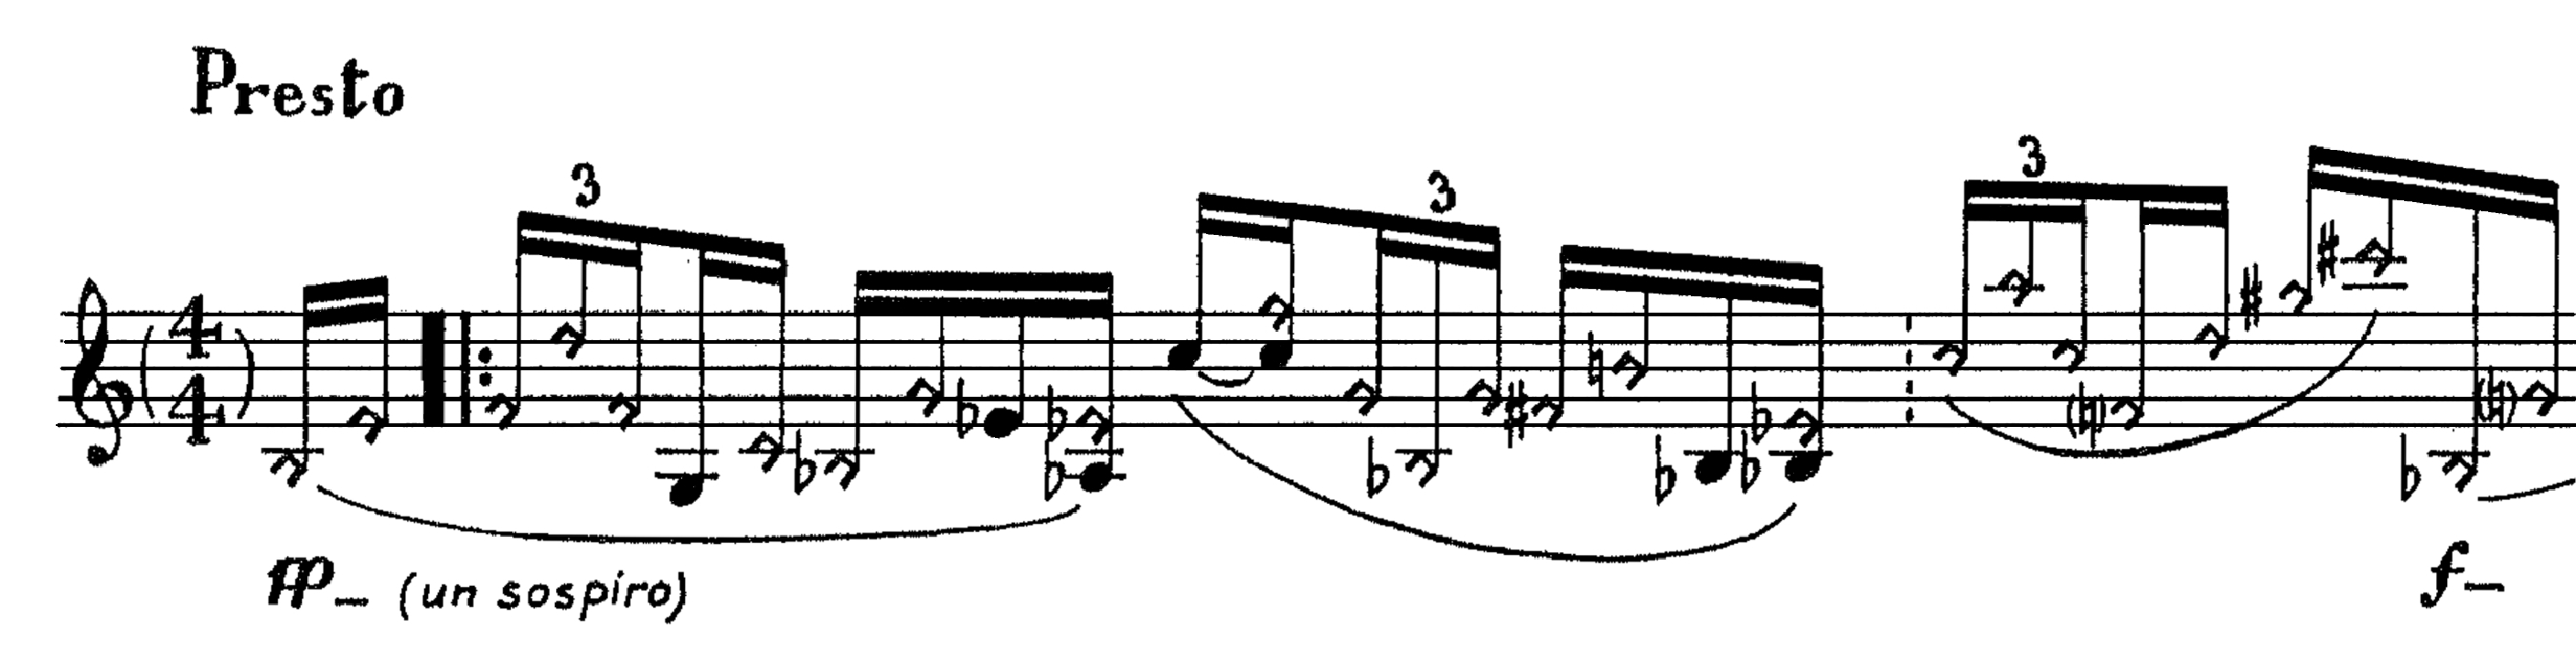
\includegraphics[width=\linewidth]{./resources/sciarrinoHalfHarmonicNotation.pdf}
  \caption{Excerpt from Sciarrino's 5th capriccio from \emph{6 Capricci for Violin}}\label{fig:sciarrinoExcerpt}\end{figure}

Sekulic adds to this quote, stating in \emph{Do you hear me?} that the stopped note ``which, as indicated, is only lightly touched, in conjunction with the flautato bowing'' to achieve half harmonics.\autocite[28]{sekulicYouHearMe2012}

In his work \emph{Es Vee Pea}, Bunk notates half-harmonics with a triangle notehead, and instructs the player to: \begin{quotation}
  `Bow very slow and lightly. The pitch should be fingered with a bit more pressure than a harmonic, but the string should not touch the fingerboard. 
  The result will be a quiet scratchy sound blended with a faint and unstable pitch'
\end{quotation}\autocite[]{bunkEsVeePea2002}

In her thesis on extended viola techniques, Kwok describes half harmonics as producing `a “flutey” sound, similar to that of \emph{sul tasto} and a natural harmonic'.\autocite[]{kwokBreakingSoundBarriers2018}

In his piece \emph{The Plate of Transition Nourishes the Chameleon Appetite}, Applebaum uses the half-harmonic technique with a half-filled diamond notehead, describing it as being `fingered lightly to produce noisy, semi-uncontrolled pitch'.\autocite[]{applebaumPlateTransitionNourishes1992}

Dimpker takes half-filled diamond noteheads found in Pröve's \emph{Firebird}, and compares it with Kagel's notation in his Streichquartett I/II.\autocite[120--121]{dimpkerExtendedNotationDepiction2012}
Dimpker notes the metrical disadvantages that half-filled diamond have, but fails to note that regular harmonics overcome the same issue with little fanfare.
The subject of transitions between half harmonic and harmonic, and half harmonic and \emph{normale} is discussed, with the conclusion that 
\begin{quotation}
  The transition from half harmonic pressure to harmonic pressure, and vice versa, could be requested by using two notes of the same pitch (one for the half harmonic and one for the harmonic stops) and connecting them by means of a legato slur.\autocite[121]{dimpkerExtendedNotationDepiction2012}
\end{quotation}
He also specifies that half harmonics `are not limited to the nodes and hence the natural harmonics, but may be executed on all fingerboard positions'.\autocite[121]{dimpkerExtendedNotationDepiction2012}

We begin to see that half-harmonics are relatively consistent throughout the literature, and although the terminology and descriptions of the resultant sound varies, there is a general consensus on what the sound should be.
There is not, however, as much consensus with regards to the notation of half-harmonics, and the binary nature of the technique seems to work against its favour, resulting in new forms of notation being constructed rather than composers using existing literature's notation to form a standardised notation system for half harmonics.
\subsection{Notation of half-harmonics in the literature}
Perhaps the most straight-forward technique covered in this exegesis, notation for half-harmonics have just a single variable of finger pressure to convey in notation.
The use of standard notation, modified to reflect the idea that the technique fits in `half way between' two well established techniques (normale and harmonics) would be ideal, conforming to Gould's ideology of maintaining uniformity.




% TODO: Add Gould reference for creating new notation - https://trello.com/c/pAR2S6wg/26-add-gould-reference-for-creating-new-notation